\documentclass[10pt,a4paper]{article}
\usepackage[utf8]{inputenc}
\usepackage{amsmath}
\usepackage{amsfonts}
\usepackage{amssymb}
\usepackage{makeidx}
\usepackage{graphicx}

\begin{document}

\section{Lineare Algebra Tutorium 1}
\begin{center}
Andrea Colarieti Tosti
\end{center}
\subsection{Aufgabe 1}
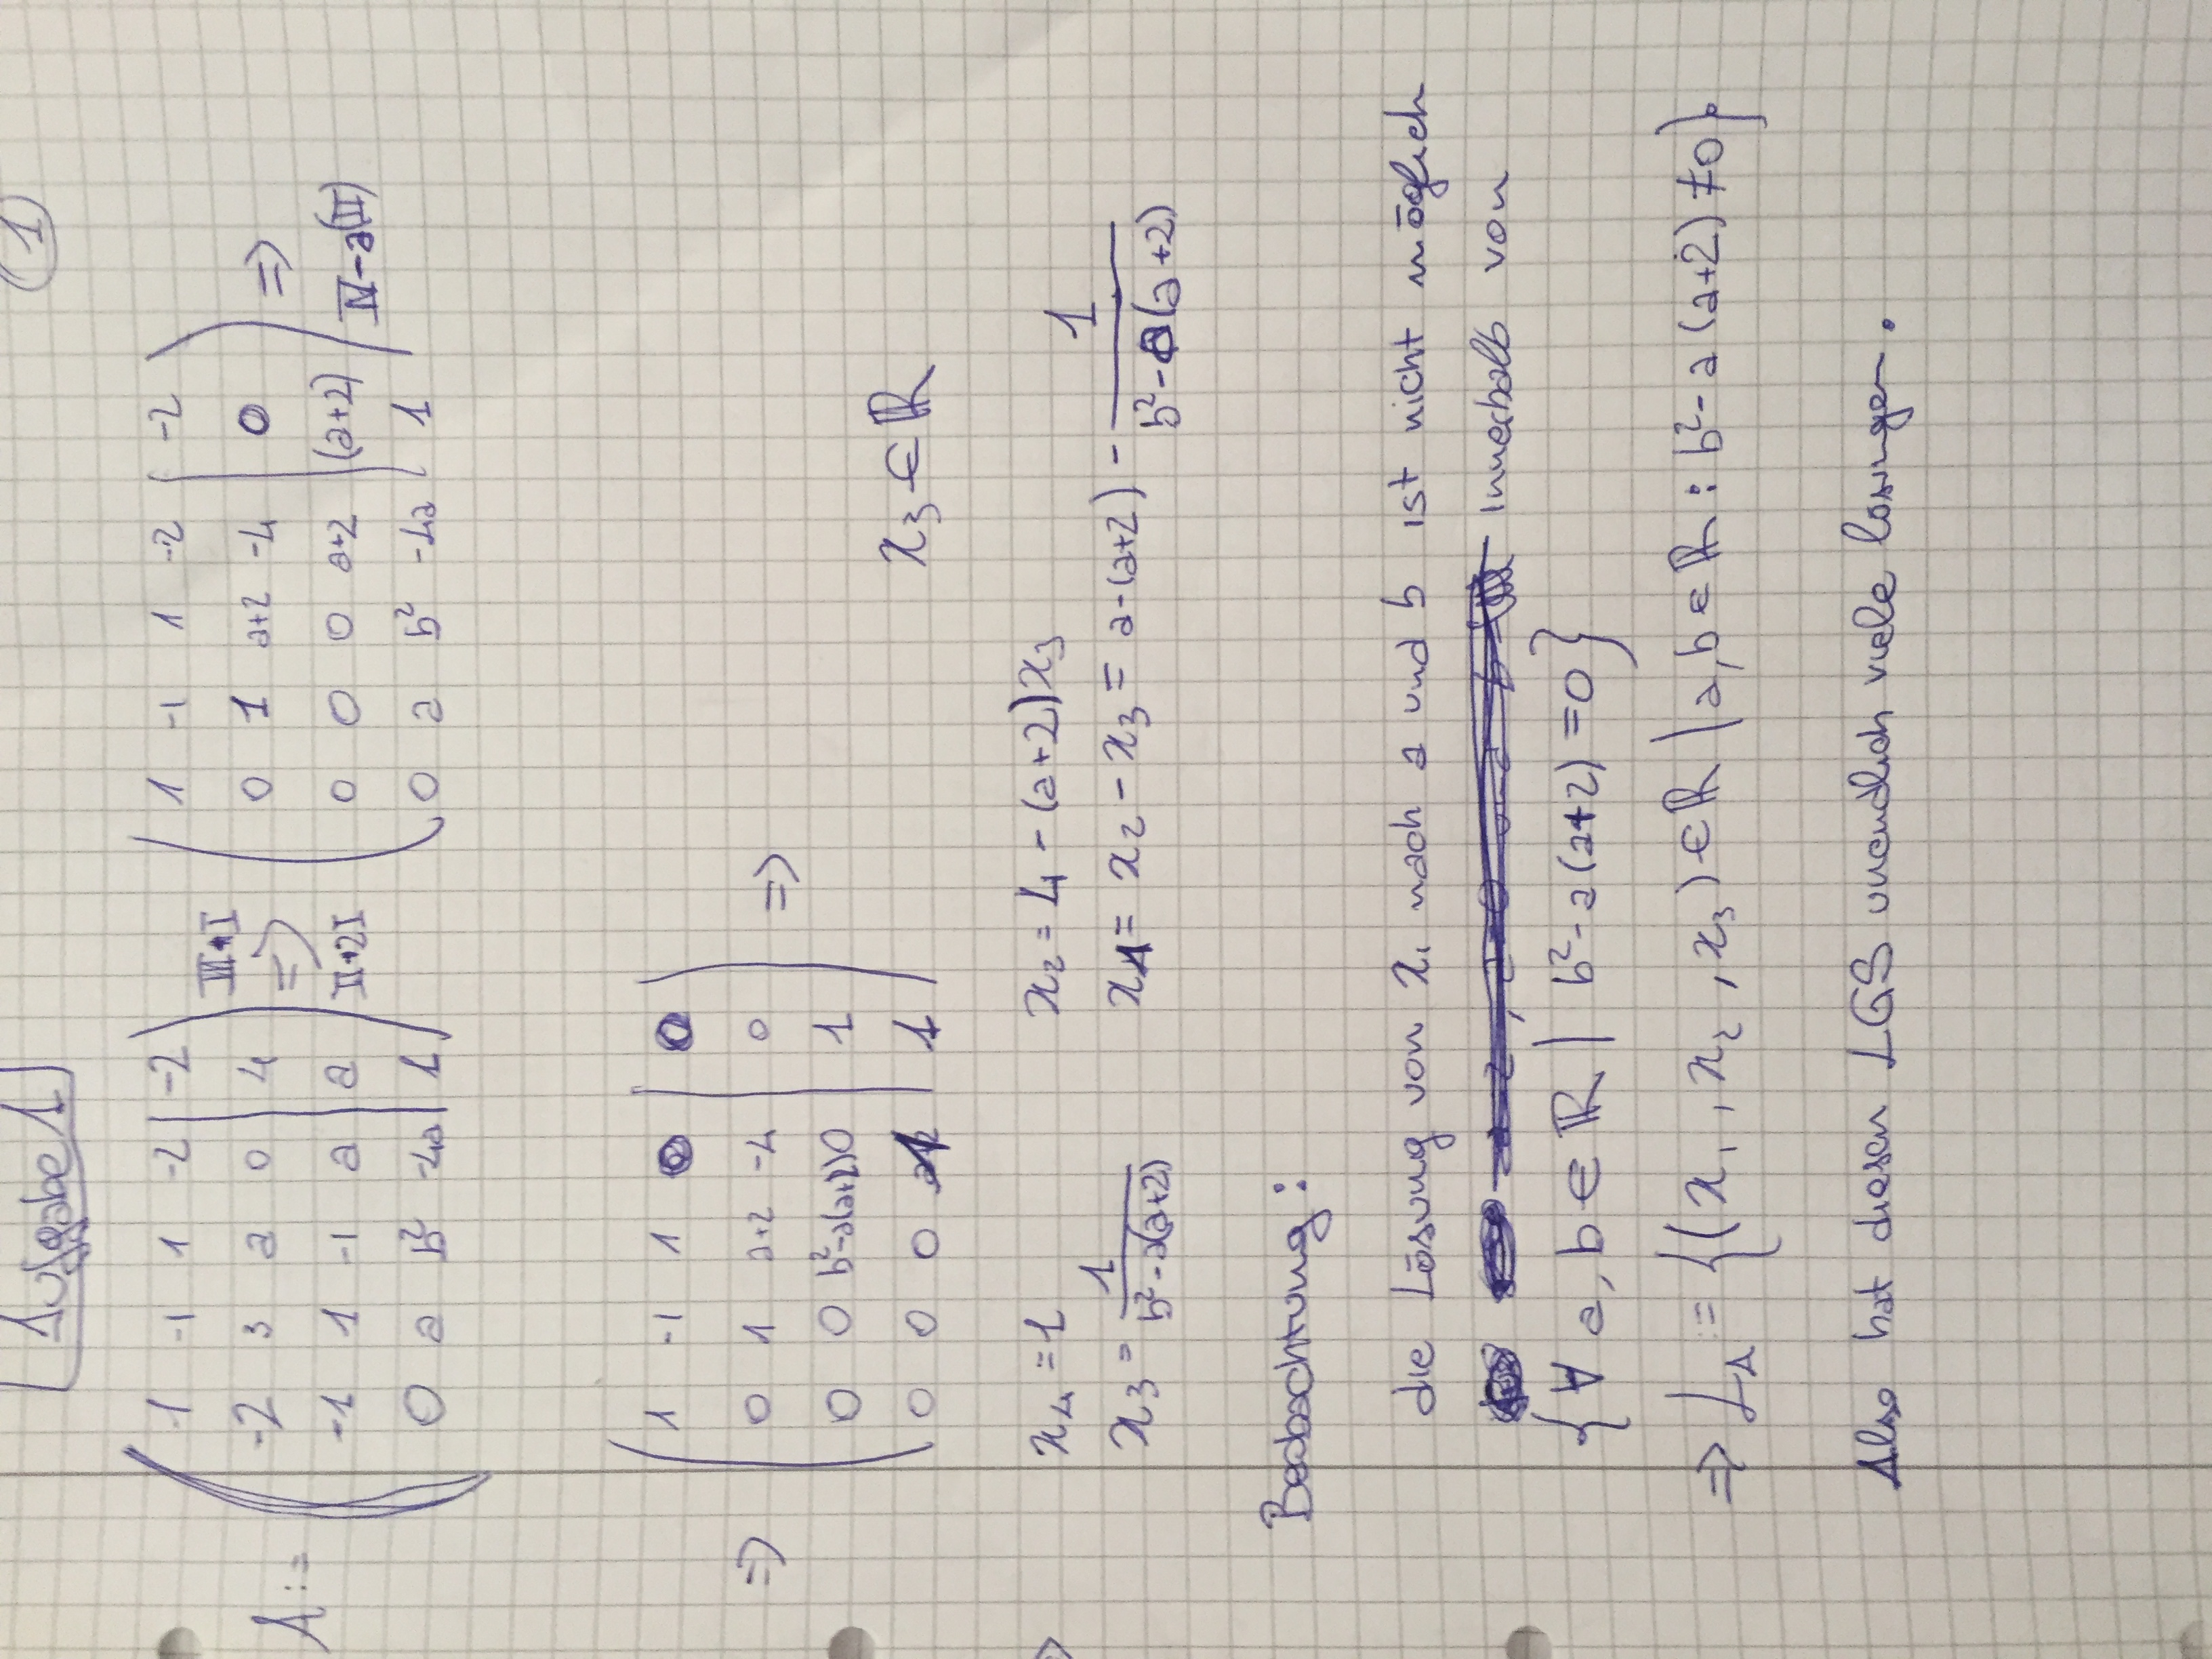
\includegraphics[scale=0.2, angle=270]{A1_1.jpg} 
\newpage
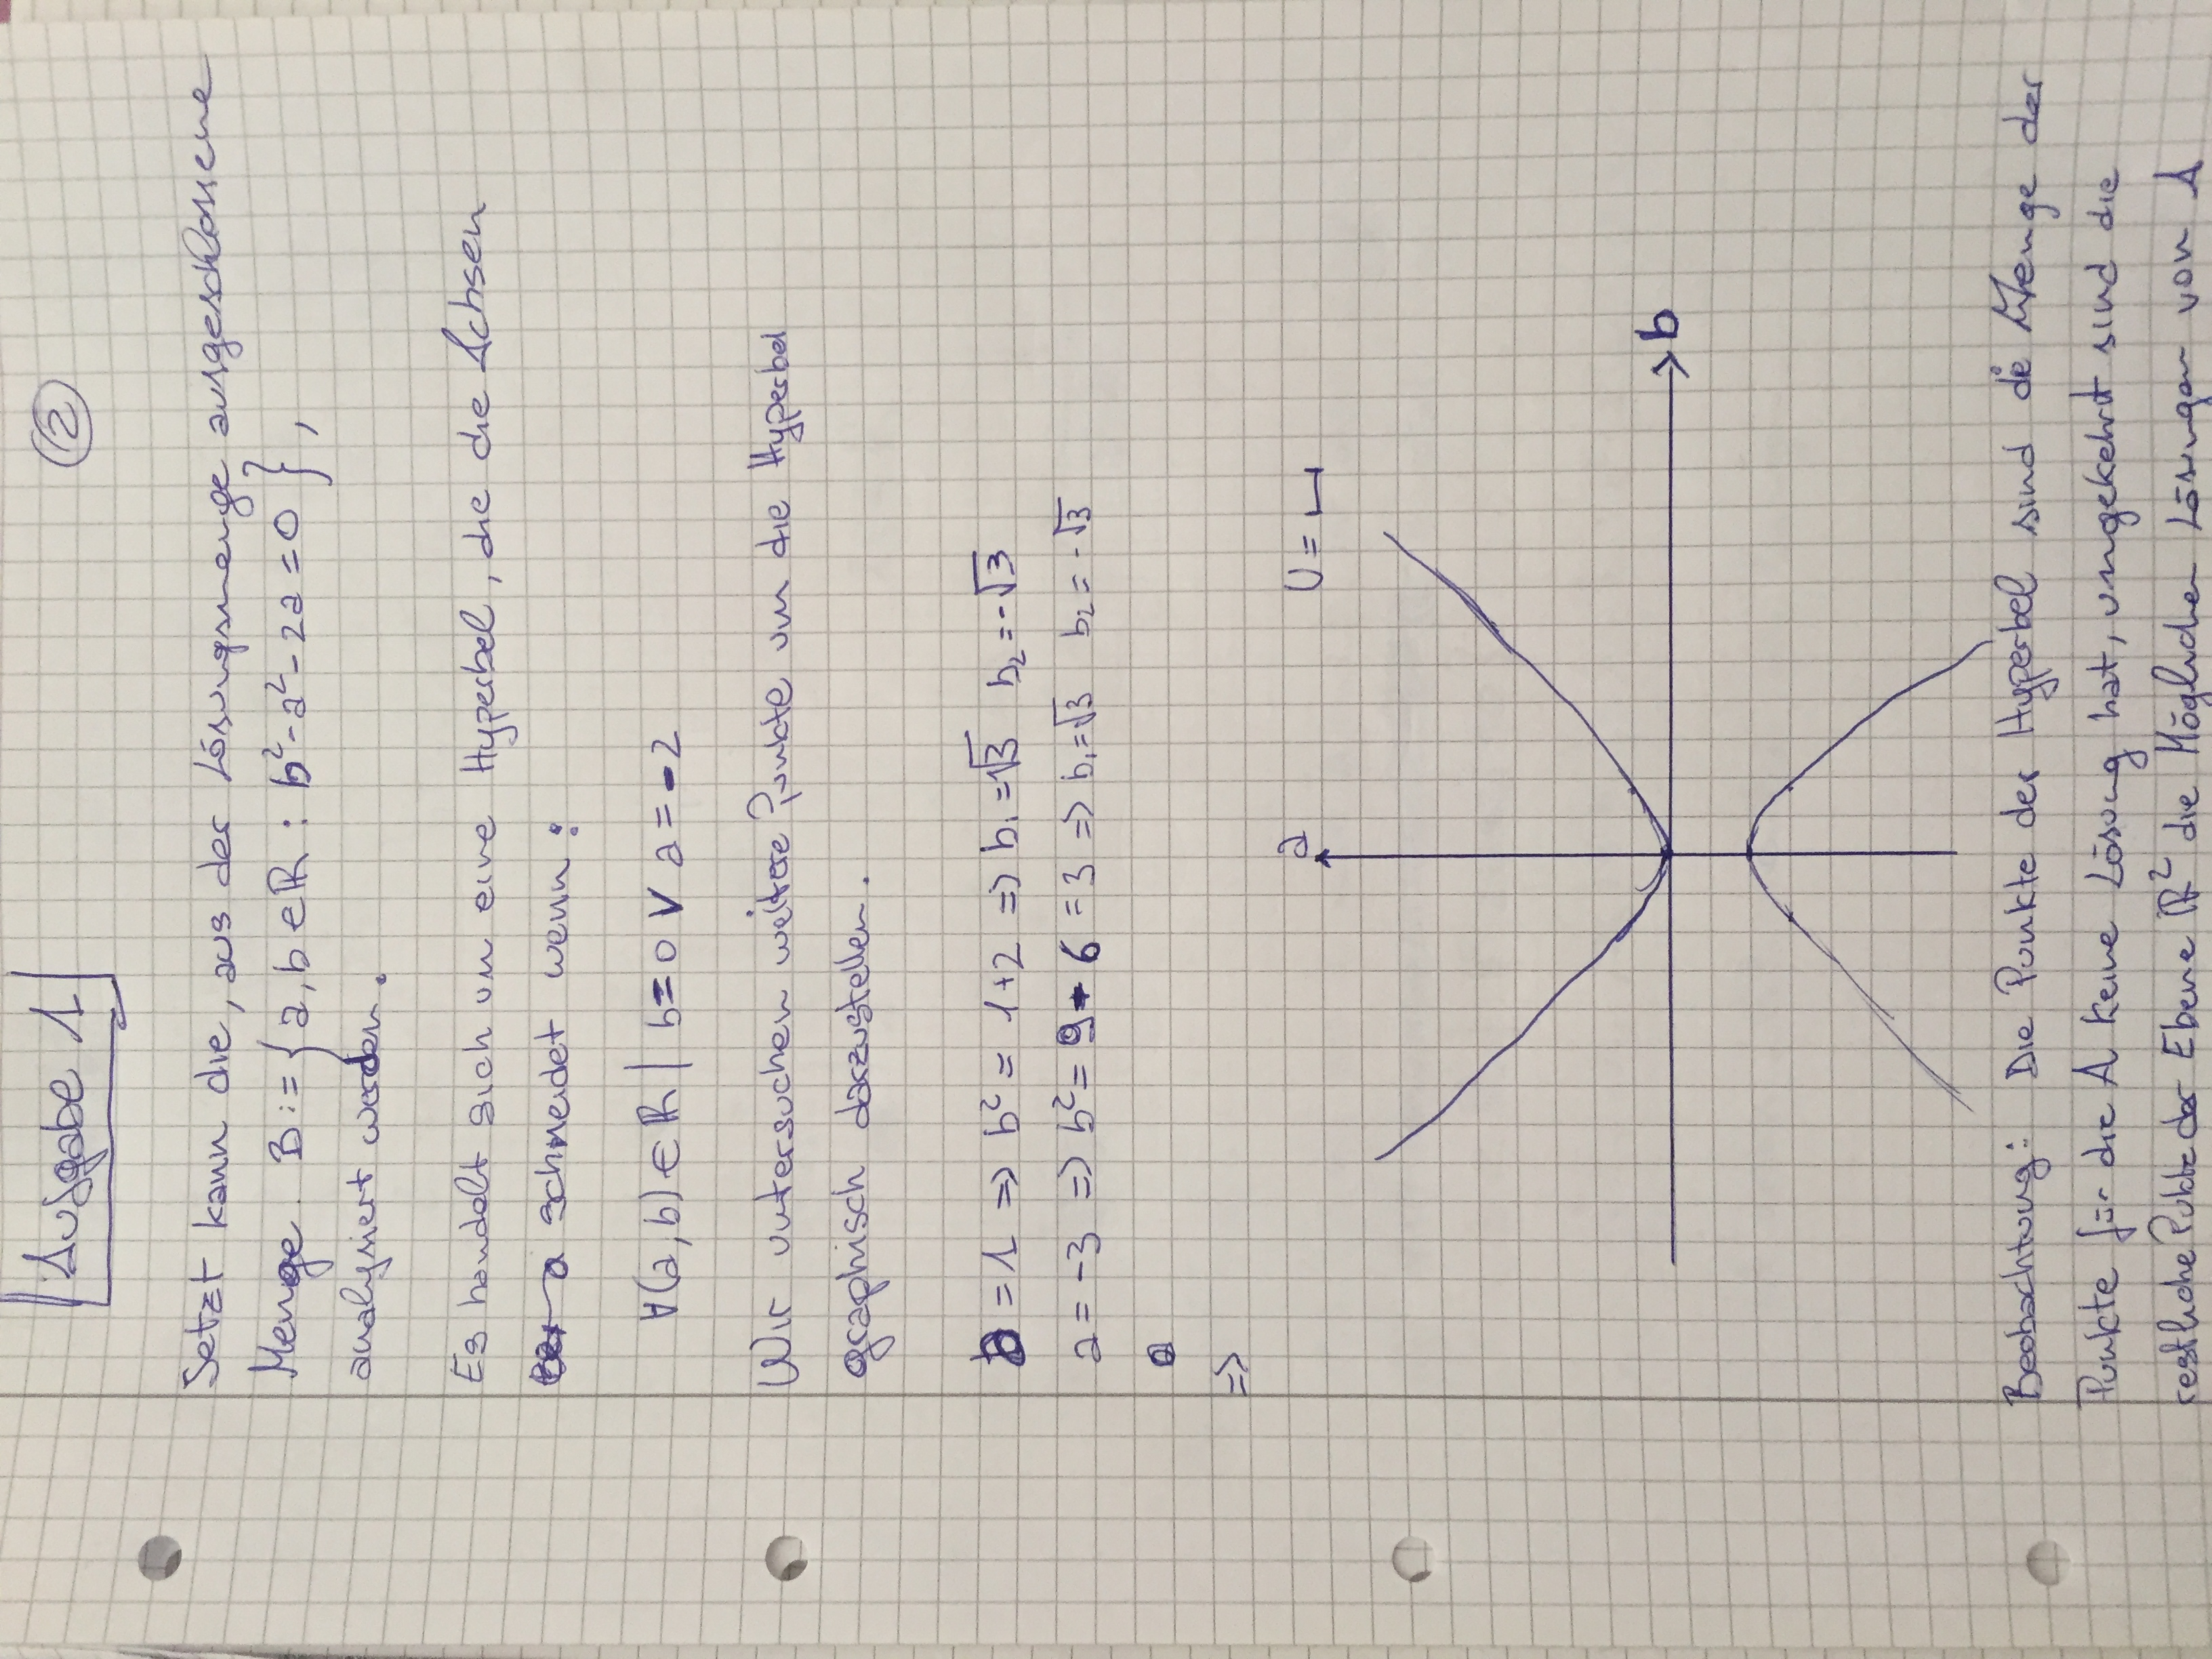
\includegraphics[scale=0.2, angle=270]{A1_2.jpg} 

\subsection{Aufgabe 2}
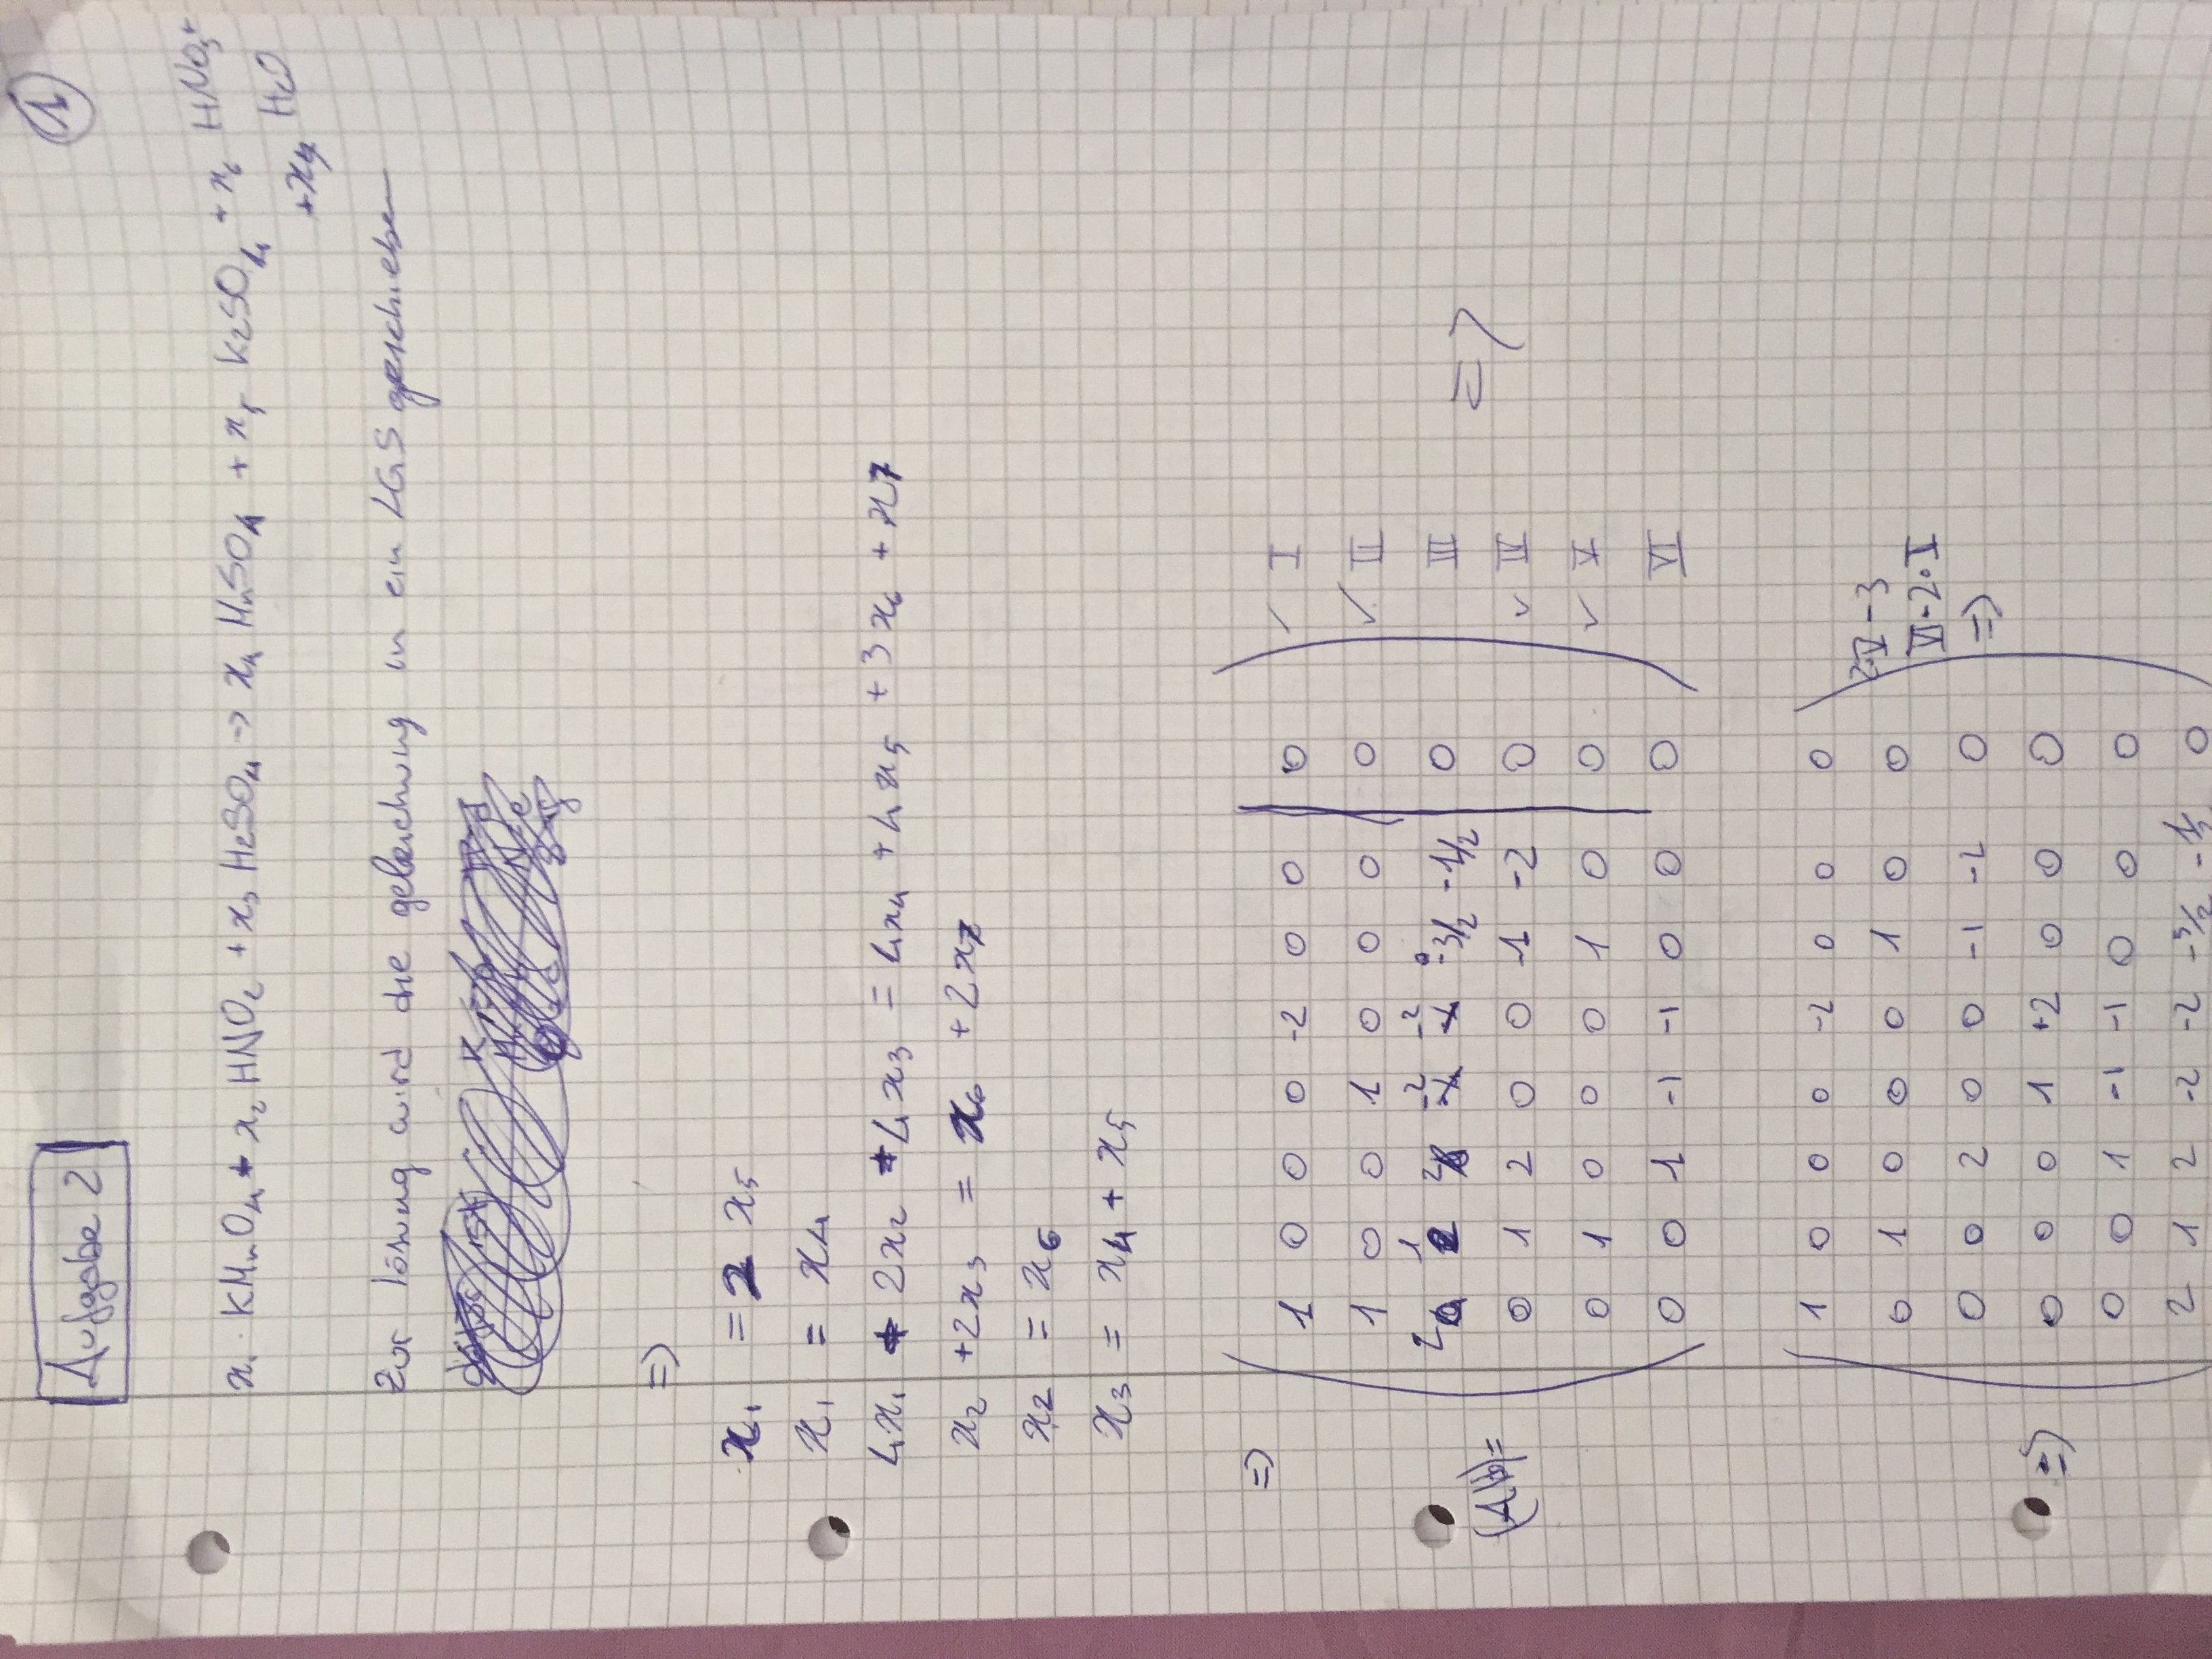
\includegraphics[scale=0.2, angle=270]{A2_1.jpg}
\newpage
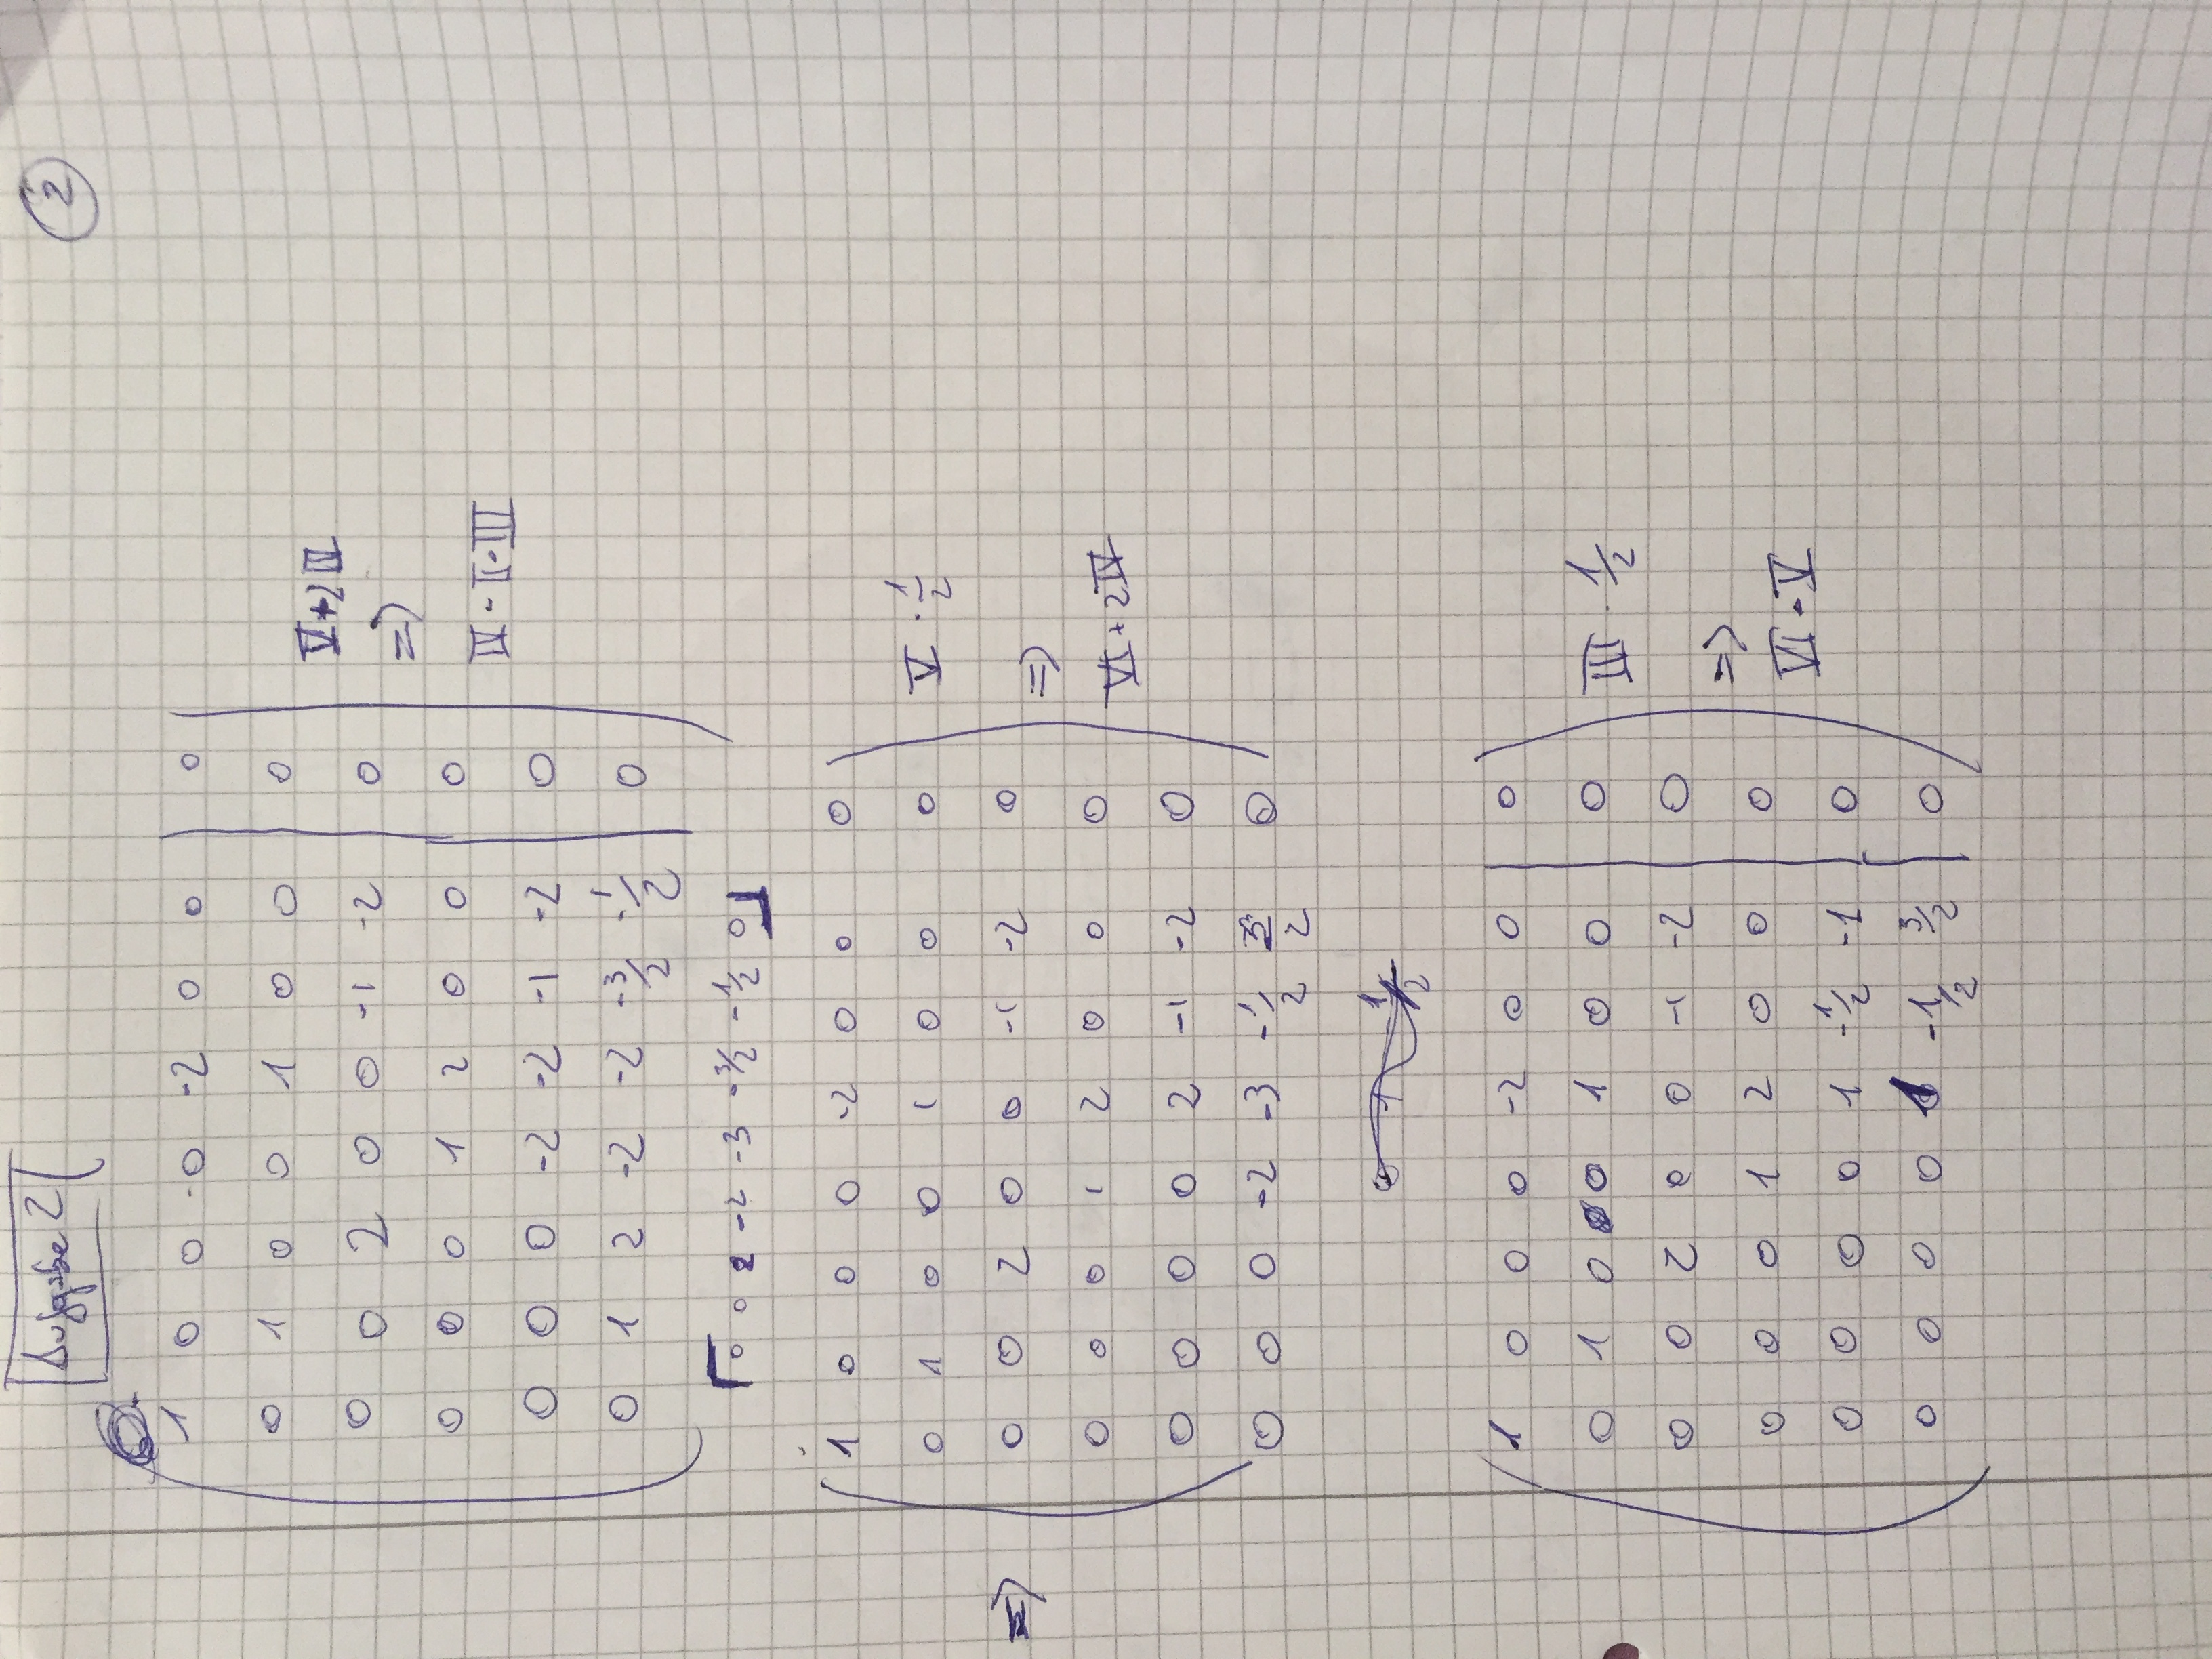
\includegraphics[scale=0.2, angle=270]{A2_2.jpg}
\newpage
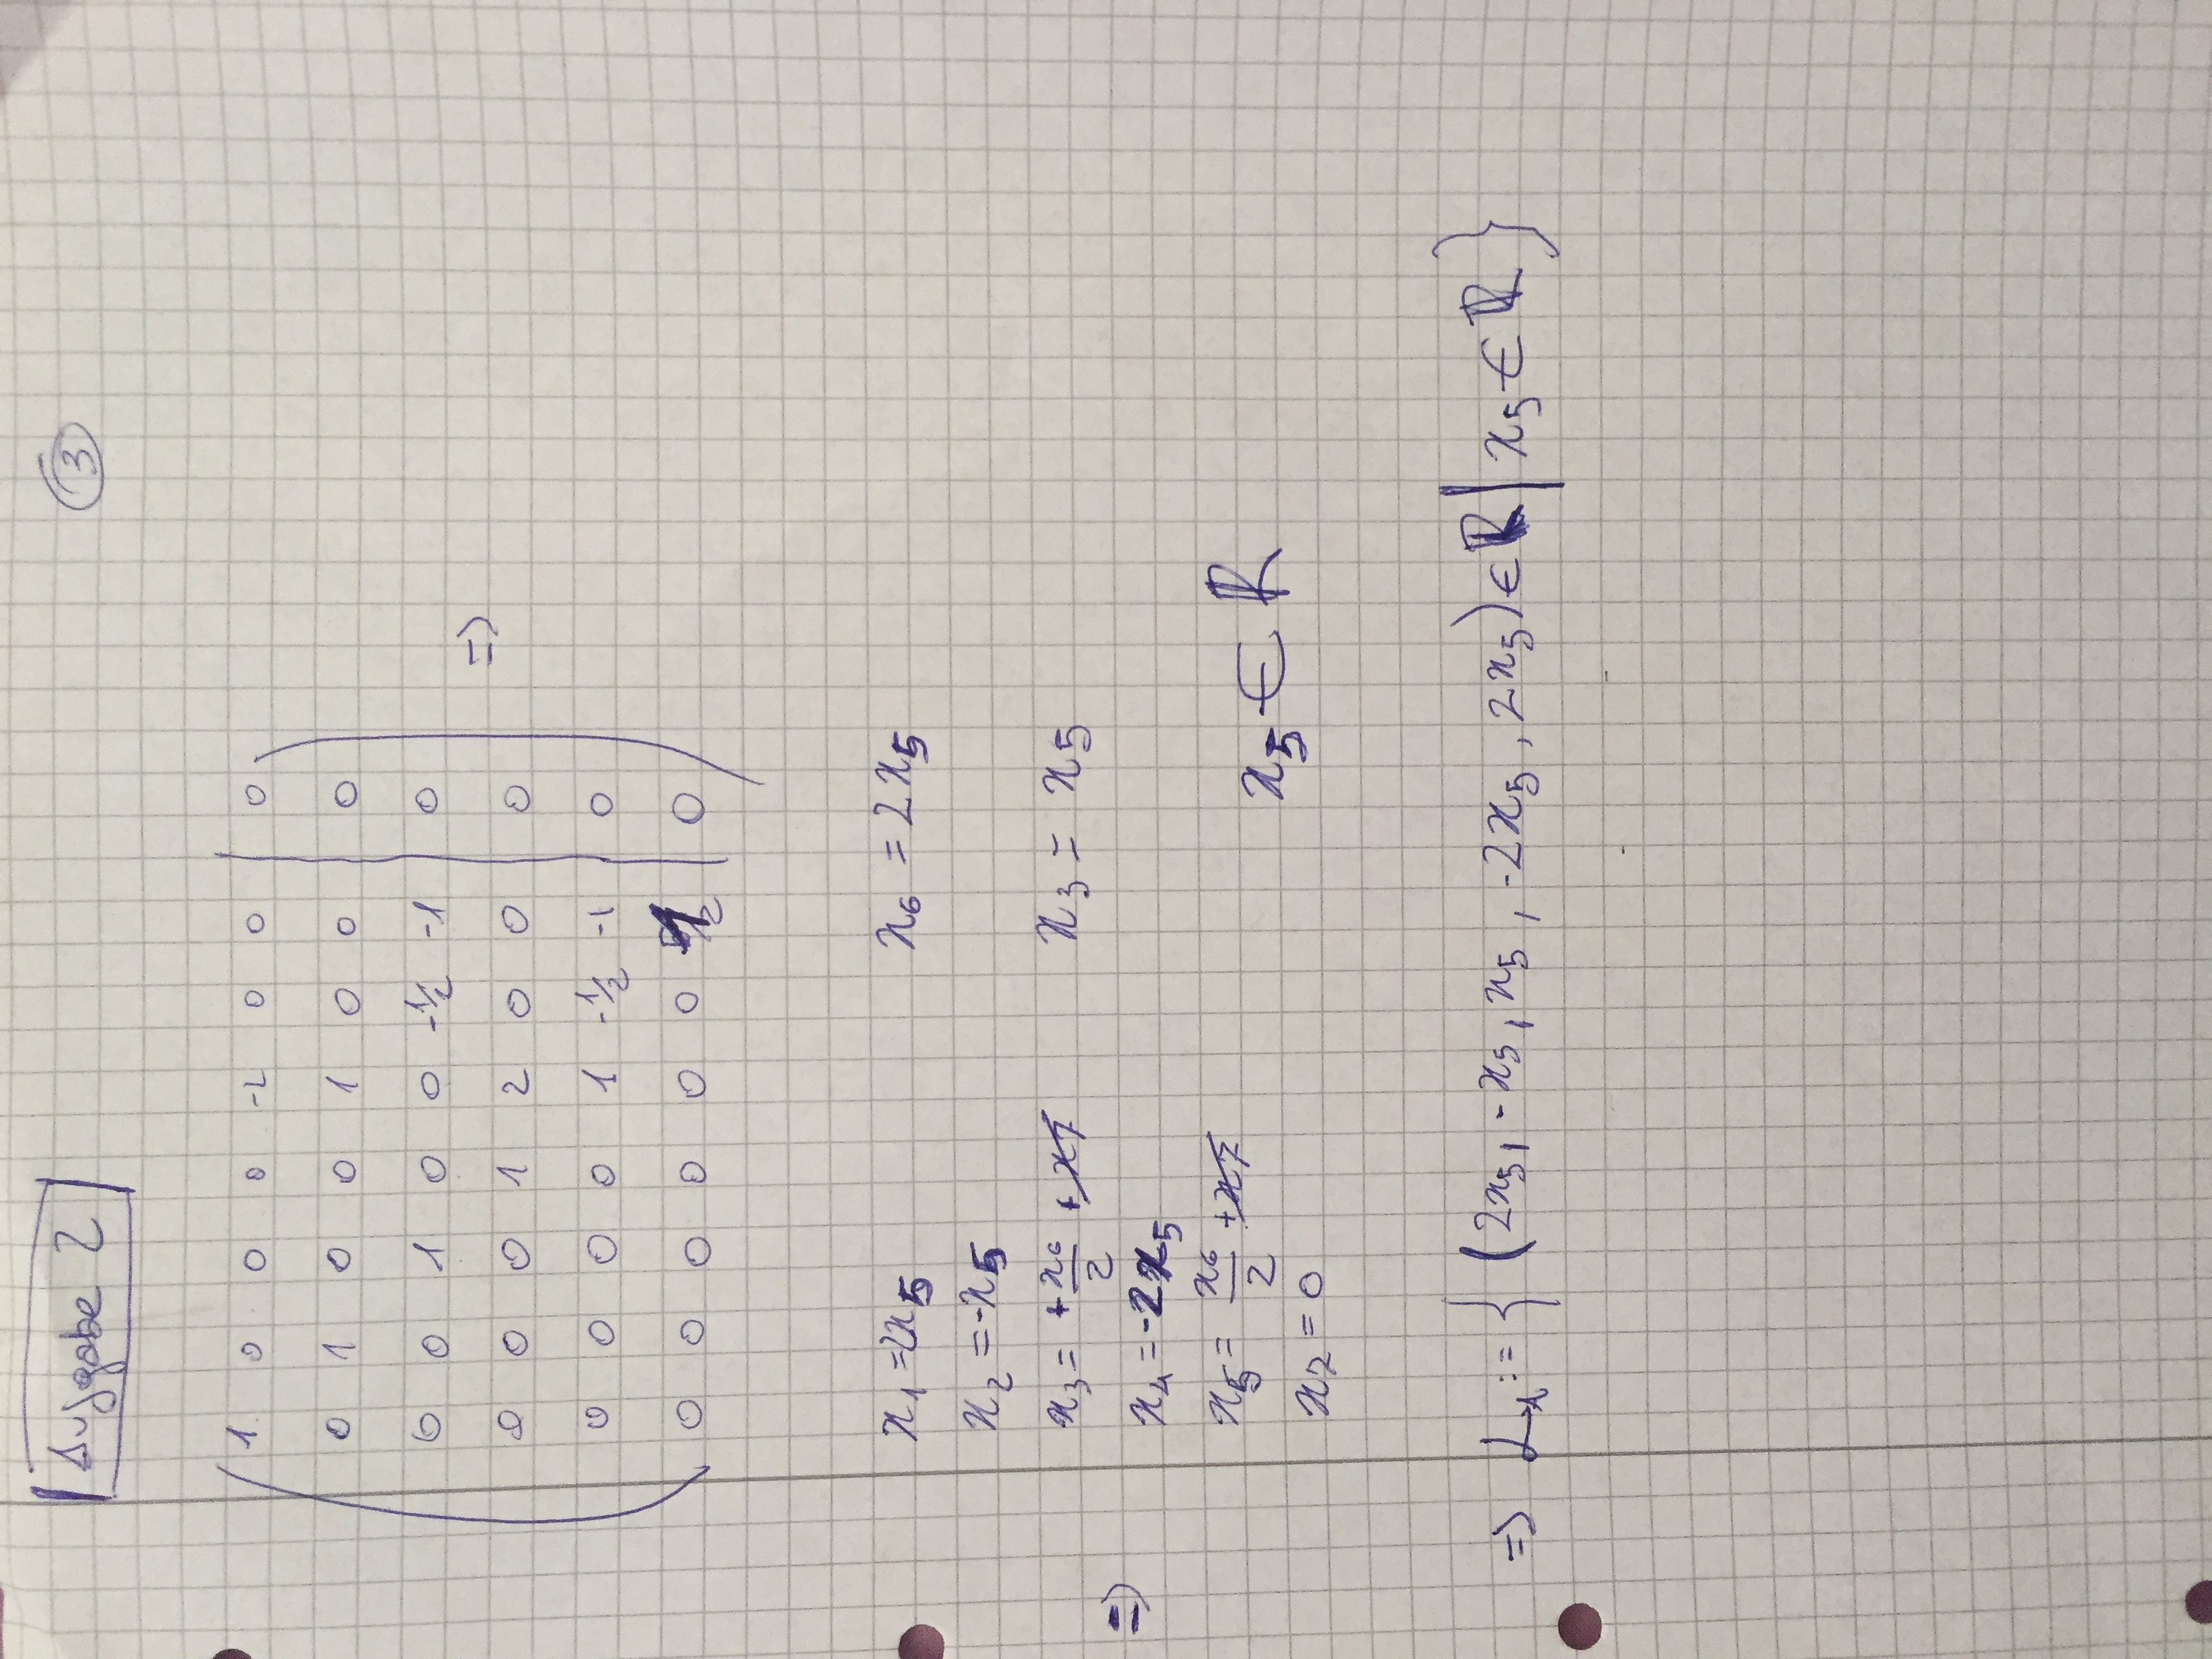
\includegraphics[scale=0.2, angle=270]{A2_3.jpg} 
\newpage


\subsection{Aufgabe 3}
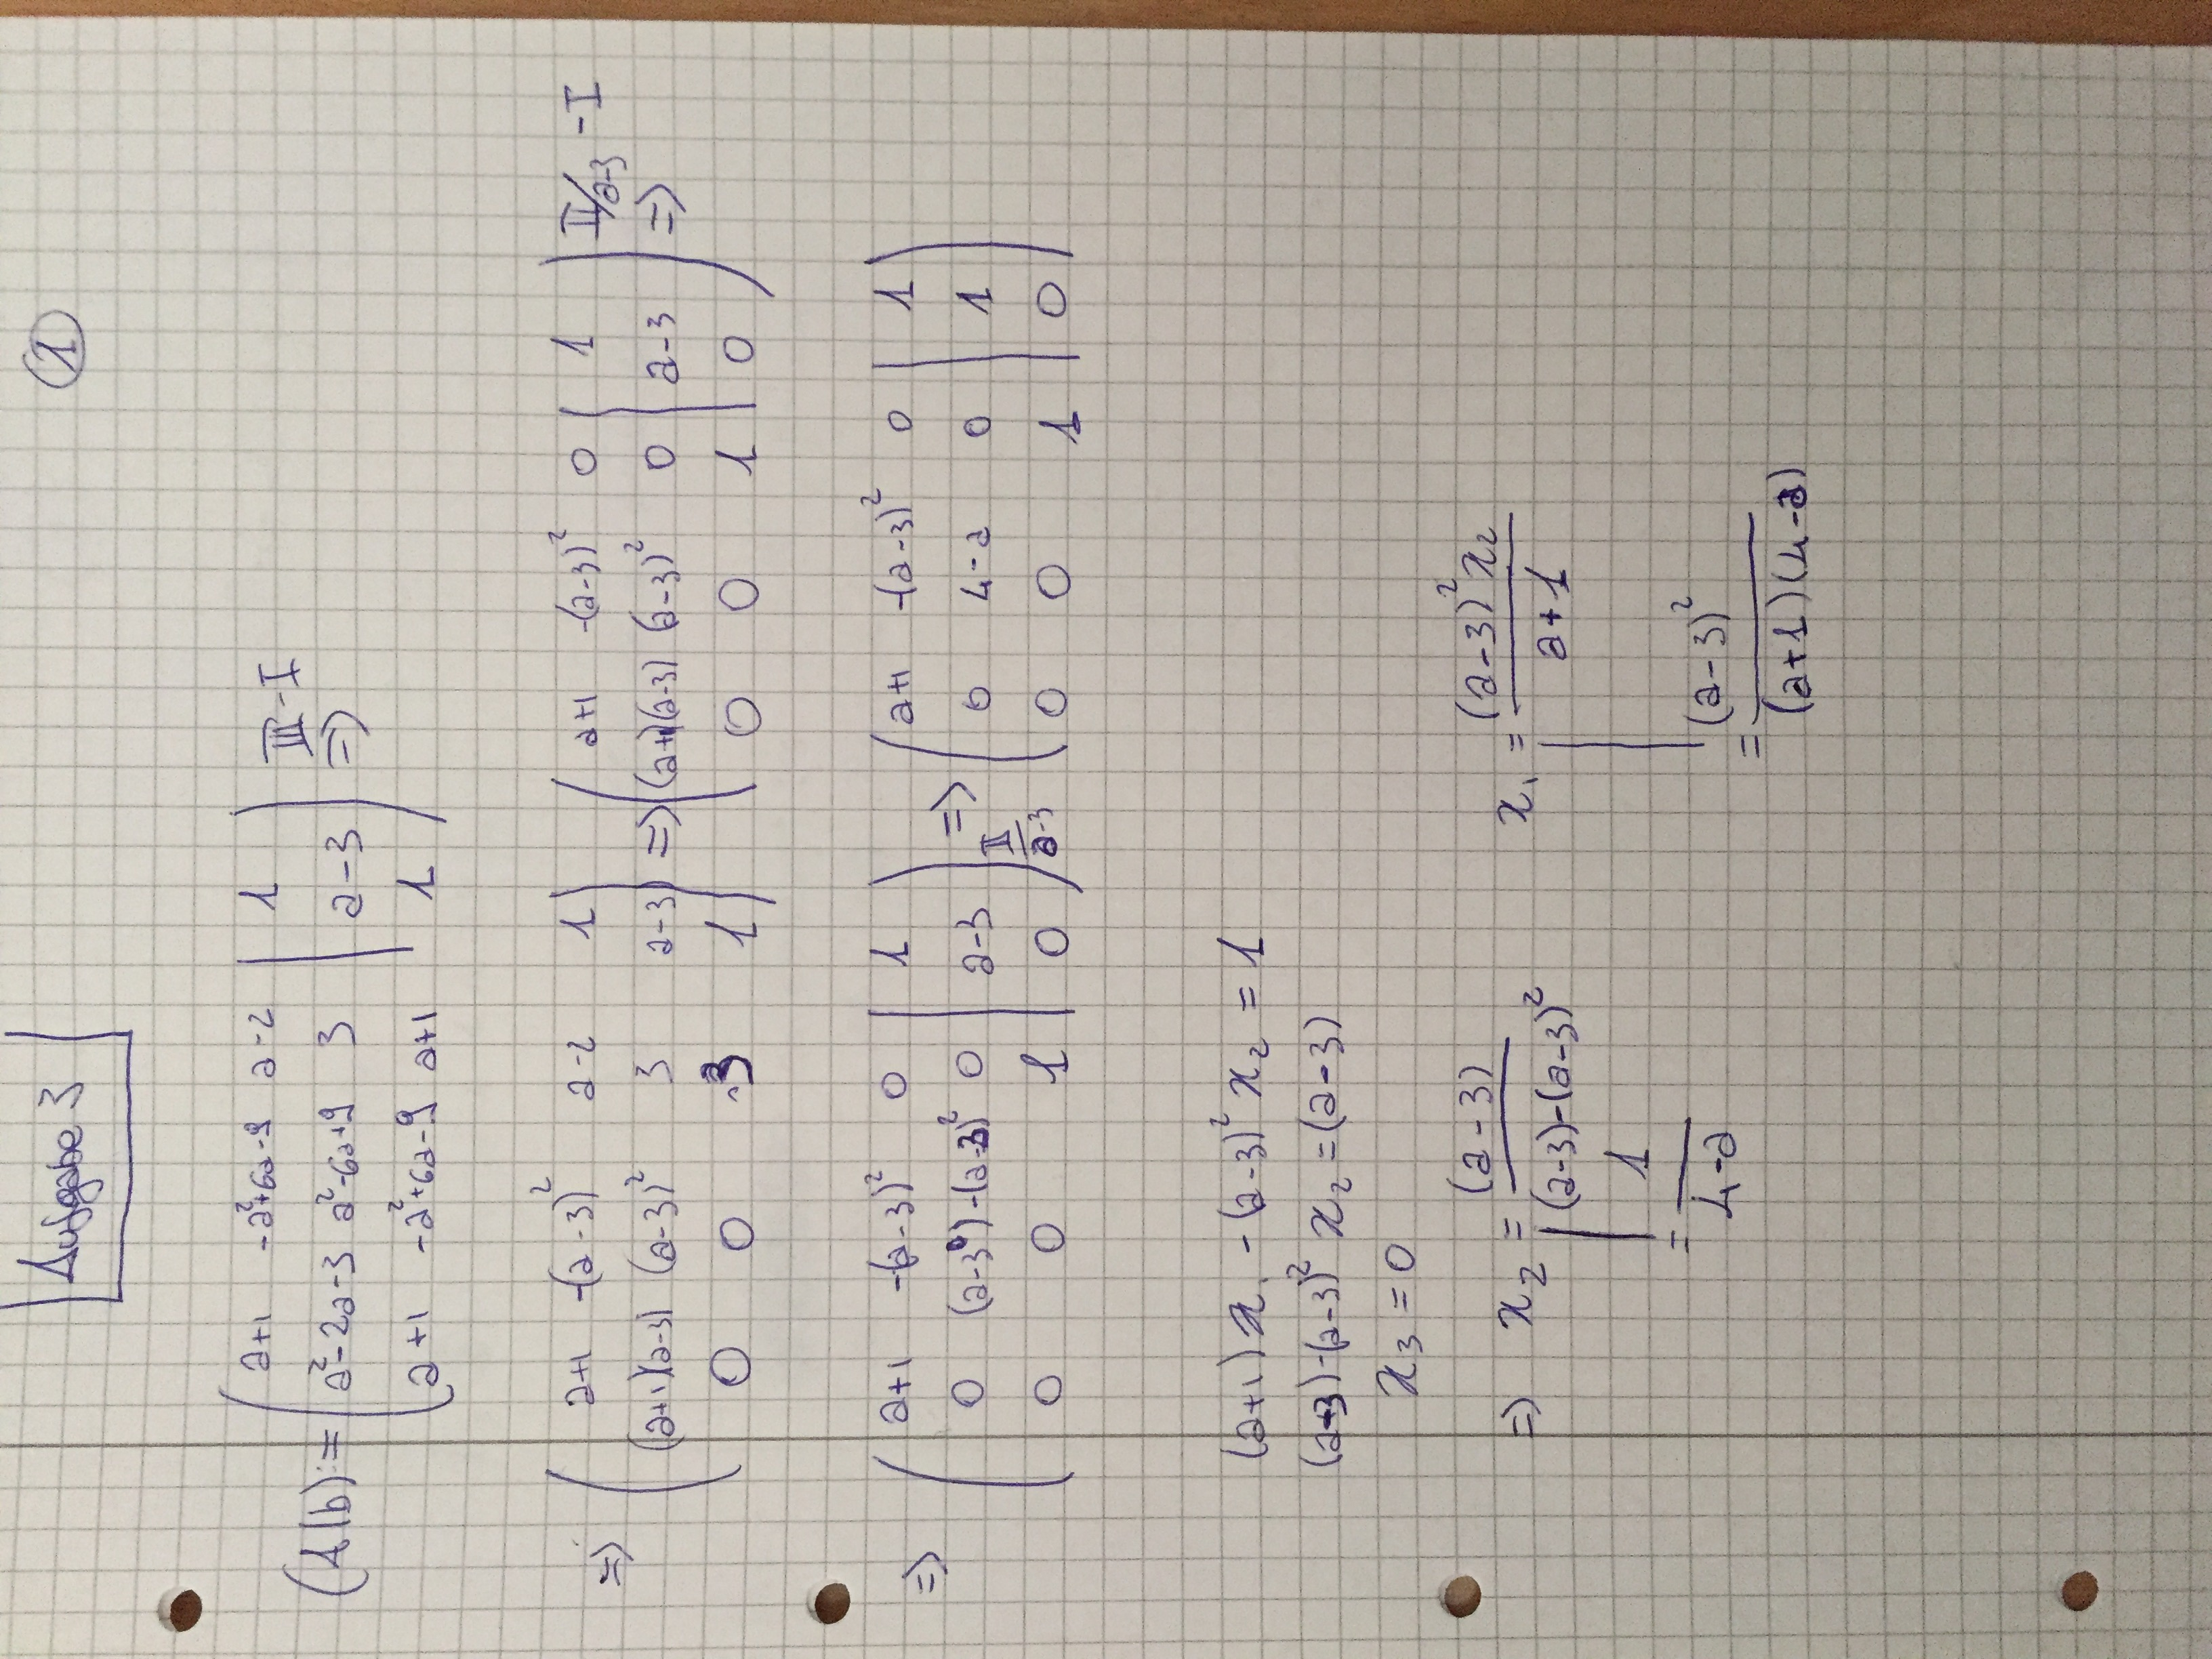
\includegraphics[scale=0.2, angle=270]{A3_1.jpg}
\newpage
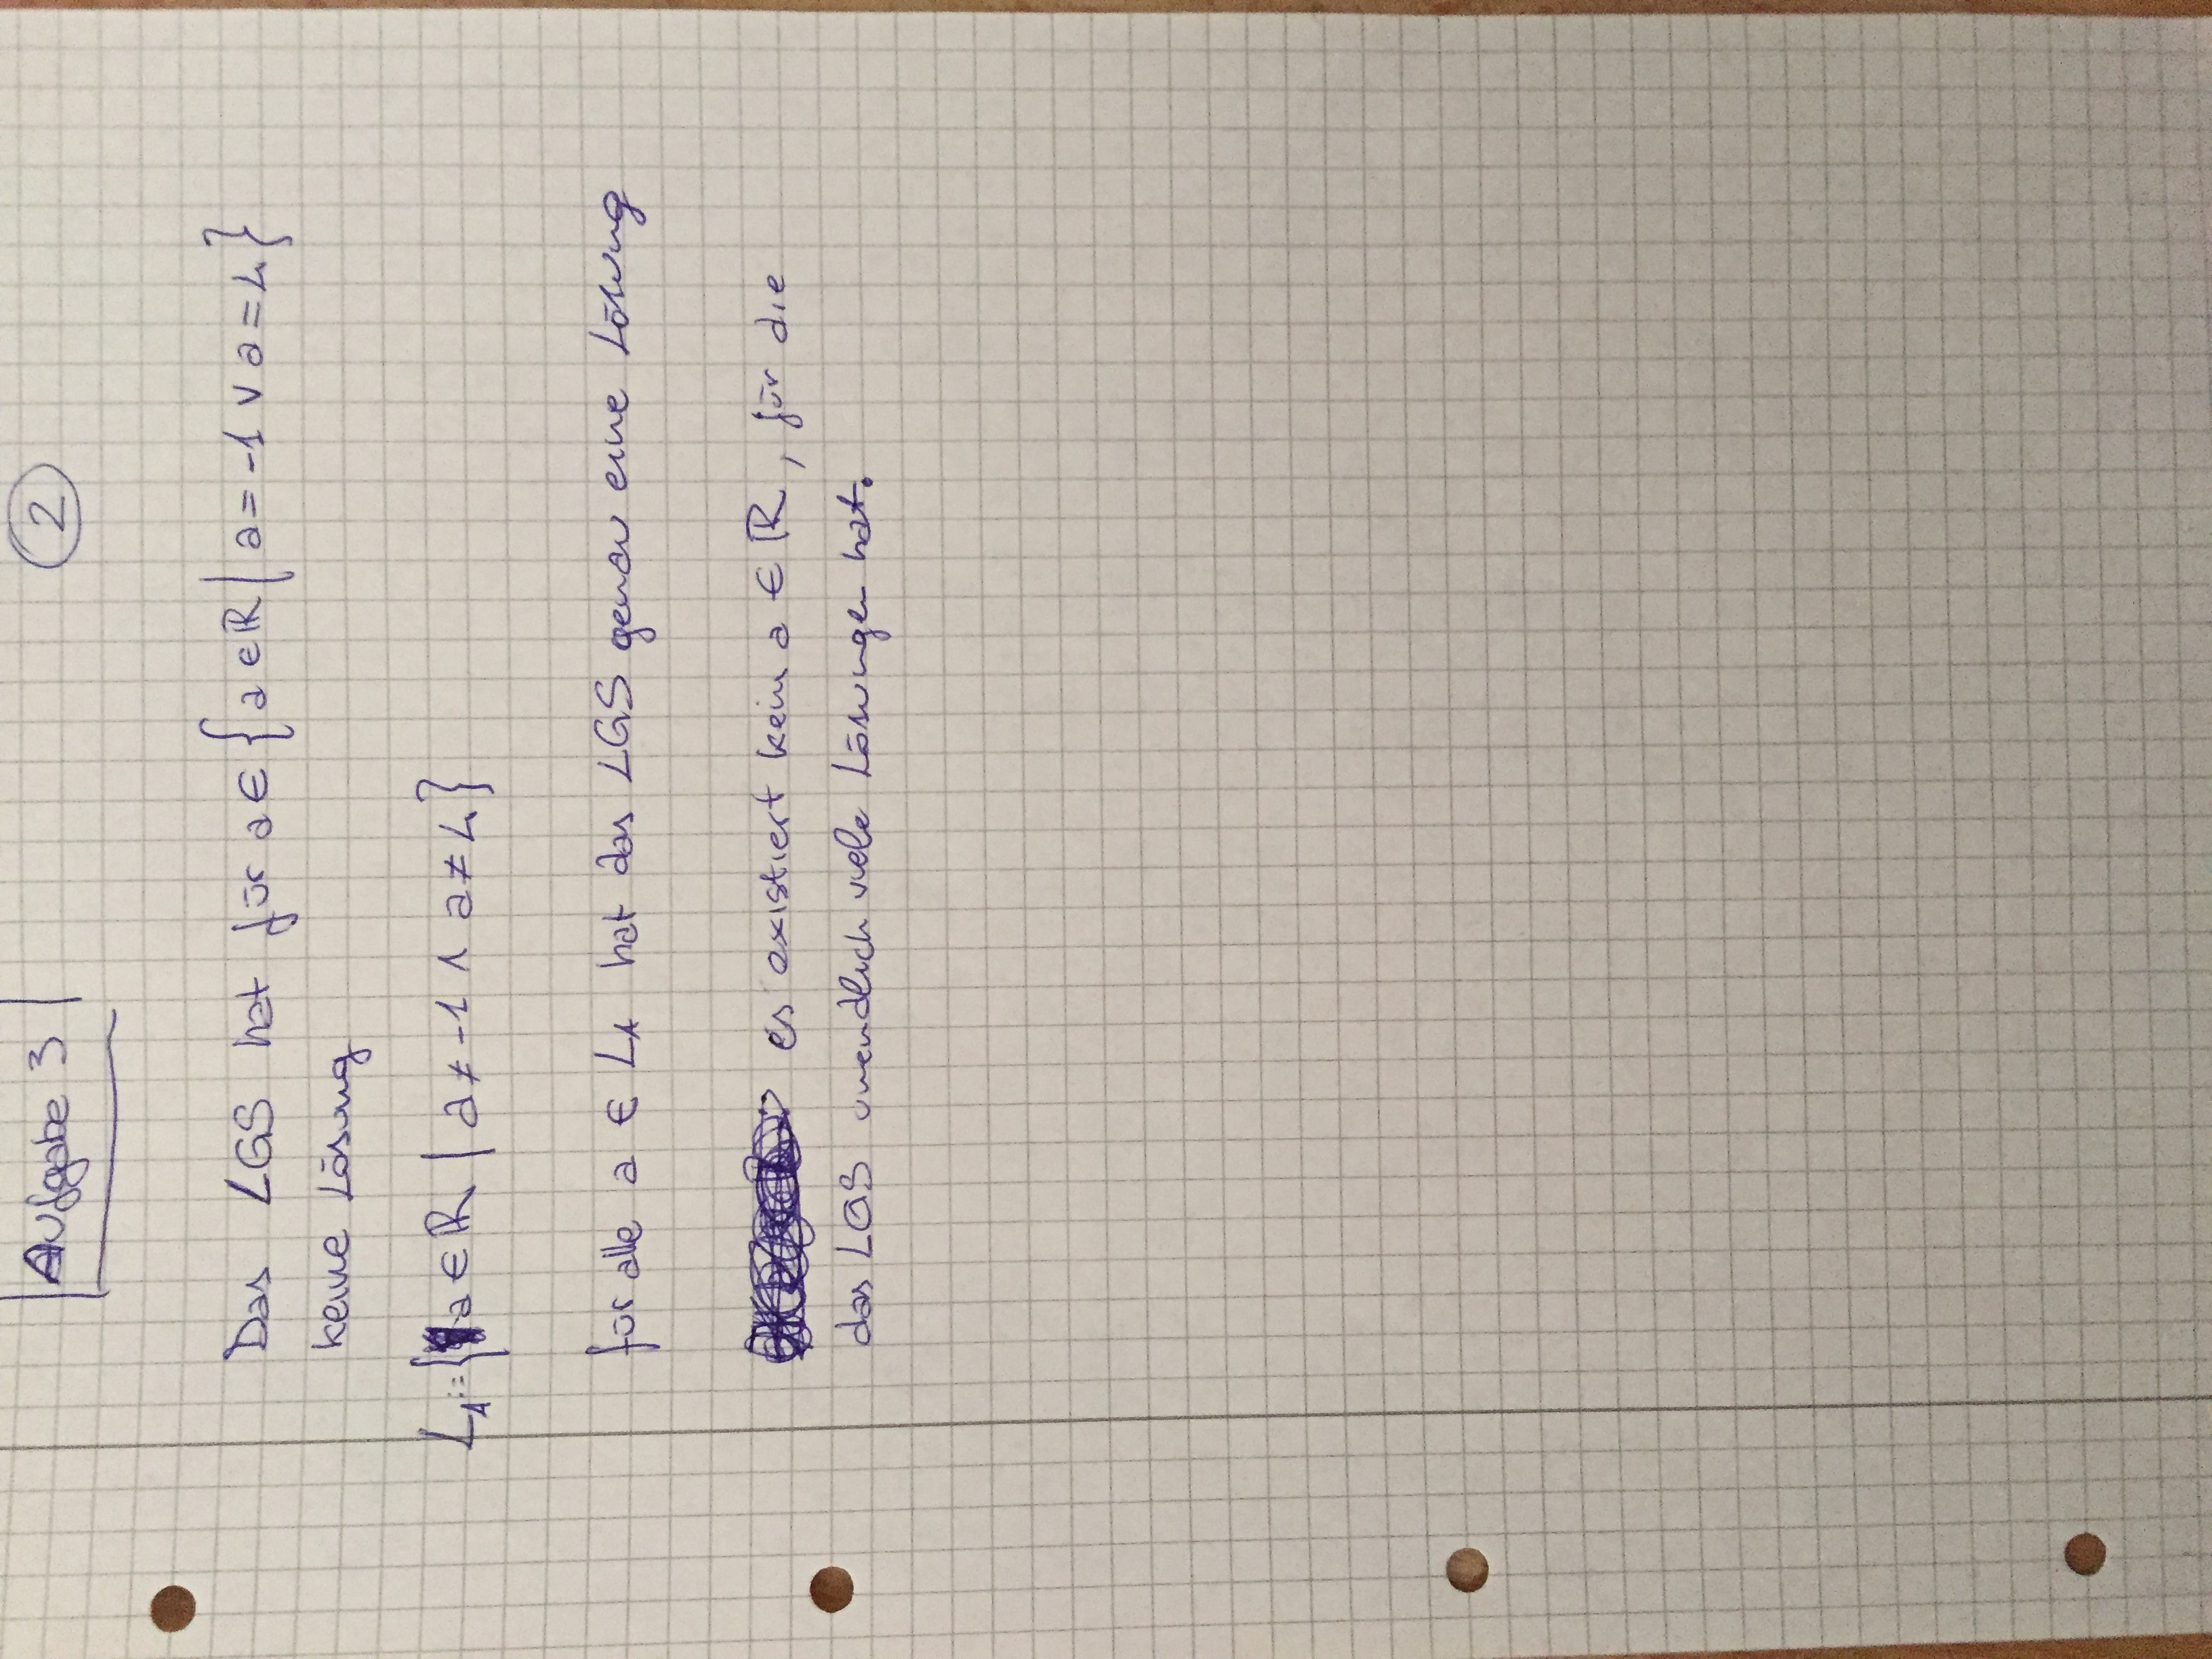
\includegraphics[scale=0.2, angle=270]{A3_2.jpg}

\subsection{Aufgabe 4}
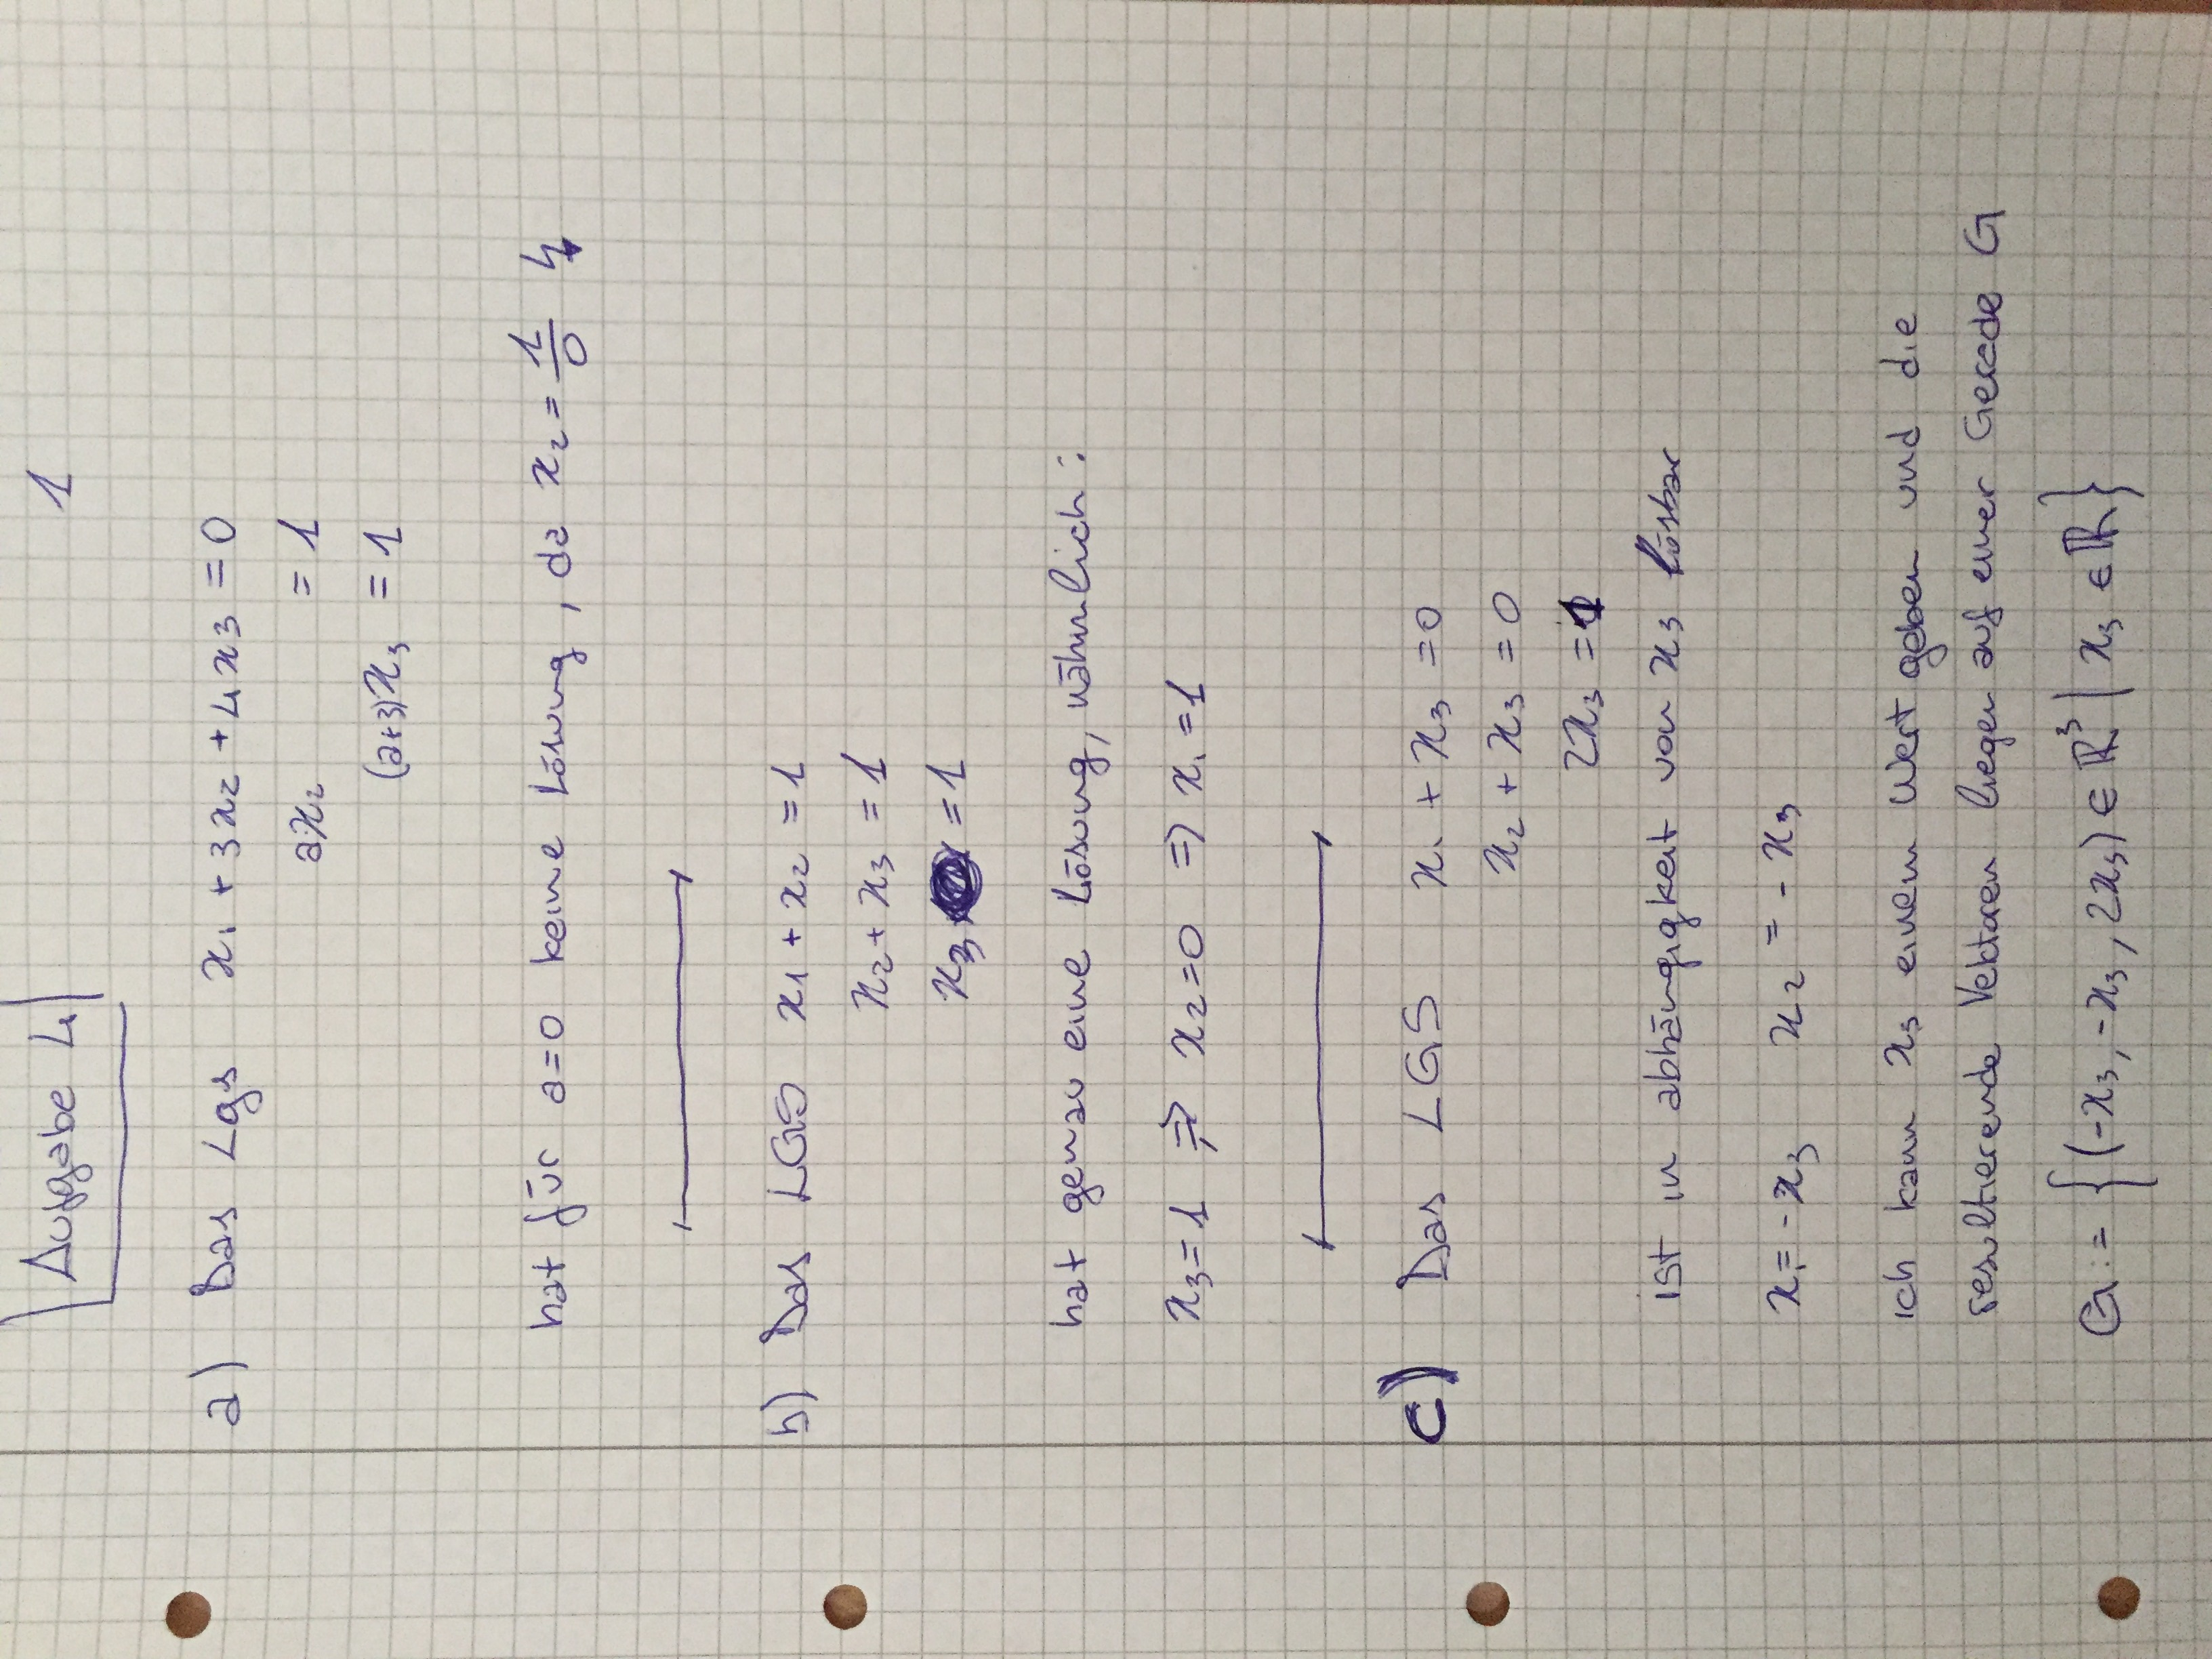
\includegraphics[scale=0.2, angle=270]{A4_1.jpg}

\end{document}